\chapter{Design of Control Model}\label{design}

\section{Proposed Control Law}\label{control_law}

Considering a flock of $k$ agents whose behaviors are described by (\ref{eq:proposed_ui}, \ref{eq:proposed_af}) in continuous time with initial positions satisfying $d_0<\|x_i(0)-x_j(0)\|^2<d_1$ for all $i\neq j$. At every time step $t$, all agents update their states with the information of the relative displacements and velocities between themselves and their neighboring agents. Compared with~\cite{CuckerDong2010}, a cohesion term is appended to the $u_i$ for the purpose of faster convergence and a more compact cohesion. We prove that when $\beta\leq\frac{1}{2}$, the velocities of agents in the flock will converge to a common value without collision with others. The regulator $\Lambda(v)$ is designed to adjust the internal repulsion and attraction forces from neighboring agents. Examples of $f_0(x), f_1(x)$ are illustrated in Fig.~\ref{fig:f0f1}.

\begin{equation}\label{eq:proposed_ui}
\begin{aligned}
\dot{x_i}(t)&=v_i(t)\\
\dot{v_i}(t)&=u_i(t)\\
u_i(t)&=\underbrace{\sum^k_{j=1}a_{ij}(x)(v_j-v_i)}_{\text{alignment term}}+\\
&\quad\underbrace{\Lambda(v)\sum_{j\neq i}f_0(\|x_i-x_j\|^2)(x_i-x_j)}_{\text{separation term}}+\\
&\quad\underbrace{\Lambda(v)\sum_{j\neq i}f_1(\|x_i-x_j\|^2)(x_j-x_i)}_{\text{cohesion term}}
\end{aligned}
\end{equation}

\begin{equation}\label{eq:proposed_af}
\begin{aligned}
a_{ij}(x)&=\frac{K}{(\sigma^2+\|x_i-x_j\|^2)^{\beta}}\\
\Lambda(v)&=(\frac{1}{k}\sum_{i>j}\|v_i-v_j\|^2)^{\frac{1}{2}}\\
f_0(x)&=\frac{1}{(x-d_0)^{\theta}}\\
f_1(x)&=\frac{1}{(x-d_1)^{\theta}}
\end{aligned}
\end{equation}

\begin{figure}[htb]
  \centering
  \subfigure[$f_0(x)$ with $d_0=1, \theta=2$]{\label{fig:f0}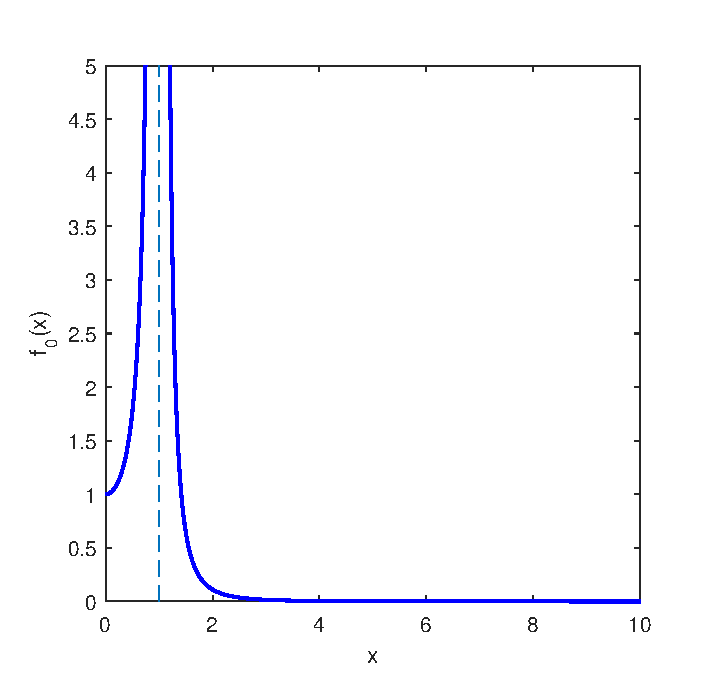
\includegraphics[width=0.48\textwidth]{figure/chapter_3/f0.eps}}
  \subfigure[$f_1(x)$ with $d_1=6, \theta=2$]{\label{fig:f1}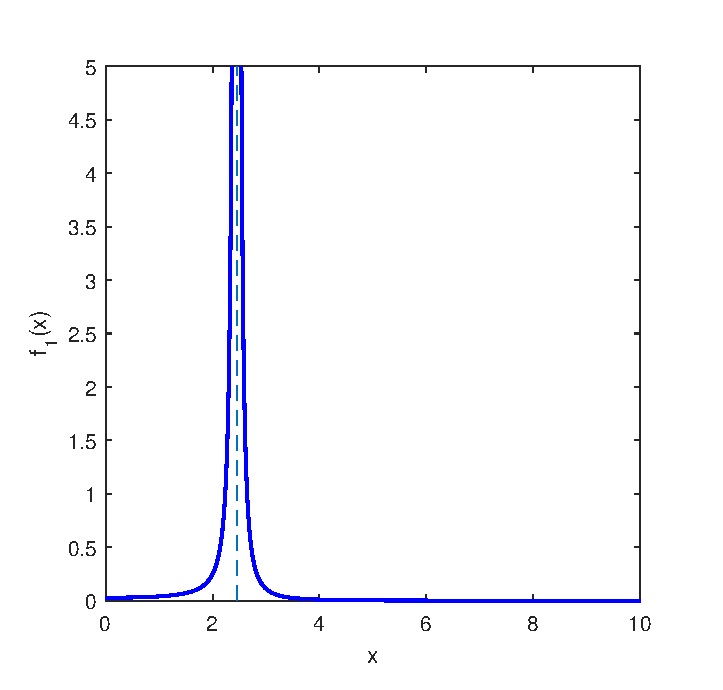
\includegraphics[width=0.48\textwidth]{figure/chapter_3/f1.eps}}
  \caption{Examples of $f_0(x), f_1(x)$ in (\ref{eq:proposed_ui}).}\label{fig:f0f1}
\end{figure}

In this flocking model, all agents are treated homogeneously that we assume each agent is identical in terms of size, mass or kinematics (\ref{eq:norminal}). For heterogeneous agents still governed by second-order dynamics with various physical characteristics, modifications in the transfer function may possible resolve this issues (\ref{eq:uncertainty}), where $\frac{k_1}{s}$ and $k_2$ represent various properties of heterogeneous agents, $\mathbf{x}$ and $\mathbf{u}$ denote the positions and control input (acceleration) respectively, and we leave this as our future works.

\begin{equation}\label{eq:norminal}
\frac{1}{s^2}=\frac{\mathbf{x}}{\mathbf{u}}
\end{equation}

\begin{equation}\label{eq:uncertainty}
\frac{1}{s^2}+\frac{k_1}{s}+k_2=\frac{\mathbf{x}}{\mathbf{u}}
\end{equation}

\section{Proof of Cohesion and Separation}

Here we omit the detailed proofs of the Lemmas and Propositions originated from~\cite{CuckerDong2010}. Let $F_f$ be the $k$ by $k$ adjacency matrix with entries $f_{ij}=f_0(\|x_i-x_j\|^2)-f_1(\|x_i-x_j\|^2)$ when $i\neq j$ and $f_{ii}=0$. Let $D_f$ be a diagonal matrix whose entries are $d_{ii}=\sum_{j=1}^k f_{ij}$. We have Laplacian matrix $L_f=D_f-F_f$. Similarly we have $L_x=D_x-A_x$, where $a_{ij}$ is defined in (\ref{eq:proposed_af}). Then (\ref{eq:proposed_ui}) could be equally defined as

\begin{equation}\label{eq:continuous}
\begin{aligned}
\mathbf{\dot{x}}&=\mathbf{v}\\
\mathbf{\dot{v}}&=-L_x\mathbf{v}+\Lambda(v)L_f\mathbf{x}\\
\end{aligned}
\end{equation}

\noindent
where $\mathbf{x}=(x_1, x_2, \dots, x_k)^T$ and $\mathbf{v}=(v_1, v_2, \dots, v_k)^T$. Noticed that matrix $L_x$ acts on $\mathbb{E}^K$ by mapping $(v_1, v_2, \dots, v_k)^T$ to $((L_x)_{i1}v_1+\dots+(L_x)_{ik}v_k)_{i\leq k}$.

Let $\{\bigtriangleup={(u, u, \dots, u)|u\in\mathbb{E}}\}$ be the diagonal of $\mathbb{E}^K$, and $\bigtriangleup^{\perp}$ be the orthogonal complement of $\bigtriangleup$ in $\mathbb{E}^K$. Then we could decompose every element $e\in\mathbb{E}^K=e_{\bigtriangleup}+e^{\perp}$ with $e_{\bigtriangleup}\in\bigtriangleup$ and $e^{\perp}\in\bigtriangleup^{\perp}$. We then decompose $\mathbf{v}=\mathbf{v_{\bigtriangleup}+v^{\perp}}$ where $\mathbf{v_{\bigtriangleup}}=(\bar{v}, \bar{v}, \dots, \bar{v})^T$, $\mathbf{v^{\perp}}=(v_1-\bar{v}, \dots, v_k-\bar{v})^T$ and $\bar{v}$ is the average velocity of all $k$ agents. We show that $\langle\mathbf{v_{\bigtriangleup}}, \mathbf{v^{\perp}}\rangle=\sum_{i=1}^k\langle\bar{v},v_i-\bar{v}\rangle=\langle\bar{v},\sum_{i=1}^k(v_i-\bar{v})\rangle=0$.

$\mathit{Lemma\ 1}$: For any solution $(\mathbf{x}(t), \mathbf{v}(t))$ of (\ref{eq:continuous}), we have $\frac{d}{dt}\mathbf{v}_{\bigtriangleup}=0$.

From Lemma 1, we know that $\mathbf{v_{\bigtriangleup}}$ is constant with $t$ and $a_{ij}(x)=a_{ij}(x^{\perp})$. Thus in the following paragraphs, we use $\mathbf{x}$ and $\mathbf{v}$ to denote $\mathbf{x}^{\perp}$ and $\mathbf{v}^{\perp}$ respectively. The system in (\ref{eq:continuous}) then becomes the following

\begin{equation}\label{eq:continuous_projection}
\begin{aligned}
\mathbf{\dot{x}}&=\mathbf{v}\\
\mathbf{\dot{v}}&=-L_x\mathbf{v}+\|\mathbf{v}\|L_f\mathbf{x}\\
\end{aligned}
\end{equation}

Define the function $E: \mathbb{E}^k\times\mathbb{E}^k\to(0,\infty)$ by (\ref{eq:Exv}), where $\delta$ is an infinitesimal positive number.

\begin{equation}\label{eq:Exv}
\begin{aligned}
E(\mathbf{x}, \mathbf{v})&=\|\mathbf{v}\|+\frac{1}{2}\sum_{i>j}\int_{\|x_i-x_j\|^2}^{d_1-\delta}f_0(r)dr-\frac{1}{2}\sum_{i>j}\int_{\|x_i-x_j\|^2}^{d_1-\delta}f_1(r)dr\\
&=\|\mathbf{v}\|+\frac{1}{2}\sum_{i>j}\int_{\|x_i-x_j\|^2}^{d_1-\delta}(f_0(r)-f_1(r))dr
\end{aligned}
\end{equation}

$\mathit{Proposition\ 1}$: For all $t>0$, $-Hk\|\mathbf{v}\|+\langle L_f\mathbf{x}, \mathbf{v}\rangle\leq\frac{d}{dt}\|\mathbf{v}\|\leq-\frac{Hk\|\mathbf{v}\|}{(1+2\|\mathbf{x}\|^2)^{\beta}}+\langle L_f\mathbf{x}, \mathbf{v}\rangle$.

$\mathit{Lemma\ 2}$: Let $A$ be a $k\times k$ positive, symmetric matrix and $L$ be its Laplacian. Then for all $u, w\in\mathbb{E}^K$ (and in particular, for all $u, w\in\bigtriangleup^{\perp}$), $\langle w, Lu\rangle=\sum_{i>j}\langle w_i-w_j, u_i-u_j\rangle a_{ij}$.

\noindent
Using Proposition 1, Lemma 2 and the fundamental theorem of calculus we see the derivative of $E$ along the solution satisfies

\begin{equation}\label{eq:dExv}
\begin{aligned}
\frac{d}{dt}E(\mathbf{x}(t), \mathbf{v}(t))&=\frac{d}{dt}\|\mathbf{v}(t)\|+\frac{1}{2}\sum_{i>j}\frac{d}{dt}\int_{\|x_i(t)-x_j(t)\|^2}^{d_1-\delta}(f_0(r)-f_1(r))dr\\
&=\frac{d}{dt}\|\mathbf{v}(t)\|-\frac{1}{2}\sum_{i>j}\frac{d}{dt}\langle x_i(t)-x_j(t),x_i(t)-x_j(t)\rangle(f_0(\|x_i(t)-x_j(t)\|^2)\\
&\quad\ -f_1(\|x_i(t)-x_j(t)\|^2))\\
&\leq-\frac{Hk}{(1+2\|\mathbf{x}\|^2)^{\beta}}\|\mathbf{v}\|+\langle L_f\mathbf{x}, \mathbf{v}\rangle-\sum_{i>j}\langle x_i-x_j, v_i-v_j\rangle(f_0(\|x_i-x_j\|^2)\\
&\quad-f_1(\|x_i-x_j\|^2))\\
&=-\frac{Hk}{(1+2\|\mathbf{x}\|^2)^{\beta}}\|\mathbf{v}\|
\end{aligned}
\end{equation}

\noindent
Hence $E(\mathbf{x}(t), \mathbf{v}(t))$ is a decreasing function of t along the solution $(\mathbf{x}(t), \mathbf{v}(t))$. Write

\begin{equation}\label{eq:E0}
E(\mathbf{x}(0), \mathbf{v}(0))=\|\mathbf{v}(0)\|+\frac{1}{2}\sum_{i>j}\int_{\|x_i(0)-x_j(0)\|^2}^{d_1-\delta}(f_0(r)-f_1(r))dr
\end{equation}

\noindent
Then for all $t\geq0$, $E(\mathbf{x}(t), \mathbf{v}(t))\leq E(\mathbf{x}(0), \mathbf{v}(0))$. This implies

\begin{equation}
\frac{1}{2}\sum_{i>j}\int_{\|x_i-x_j\|^2}^{d_1-\delta}(f_0(r)-f_1(r))dr<E(\mathbf{x}(0), \mathbf{v}(0))
\end{equation}

\noindent
From the definition of $f_0$ and $f_1$ and the initial conditions that we have ensured $d_0<\|x_i(t)-x_j(t)\|^2<d_1$ for all $i\neq j$ and $t\geq0$, otherwise the integral in (\ref{eq:Exv}) will go to infinity.

\section{Proof of Velocity Convergence}

Here, we show the proof for the case $\beta\leq\frac{1}{2}$, as the proof for $\beta>\frac{1}{2}$ is similar. From (\ref{eq:dExv}) we could obtain (\ref{eq:Et_E0}, \ref{eq:intE0})

\begin{equation}\label{eq:Et_E0}
E(\mathbf{x}(t), \mathbf{v}(t))-E(\mathbf{x}(0), \mathbf{v}(0))\leq-\int_0^t\frac{Hk}{(1+2\|\mathbf{x}(s)\|^2)^{\beta}}\|\mathbf{v}(s)\|ds
\end{equation}

\begin{equation}\label{eq:intE0}
\int_0^t\frac{Hk}{(1+2\|\mathbf{x}(s)\|^2)^{\beta}}\|\mathbf{v}(s)\|ds\leq E(\mathbf{x}(0), \mathbf{v}(0))
\end{equation}

$\mathit{Proposition\ 2}$: For all $t>0$, $\frac{d}{dt}\|\mathbf{x}(t)\|\leq\|\mathbf{v}(t)\|$.

By Proposition 2, we have

\begin{equation}\label{eq:proposition2}
\frac{d}{dt}\|\mathbf{x}(t)\|\leq\|\mathbf{v}(t)\|
\end{equation}

\begin{equation}
\int_{\|x(0)\|}^{\|x(t)\|}\frac{Hk}{(1+2y^2)^{\beta}}dy\leq E(\mathbf{x}(0), \mathbf{v}(0))
\end{equation}

\begin{equation}
\begin{aligned}
E(\mathbf{x}(0), \mathbf{v}(0))&\geq\int_{\|x(0)\|}^{\|x(t)\|}\frac{Hk}{(1+2y^2)^{\beta}}dy\geq\int_{\|x(0)\|}^{\|x(t)\|}\frac{Hky}{(1+2y^2)^{\beta+\frac{1}{2}}}dy\\
&=\left\{\begin{array}{rcl}\frac{Hk}{2-4\beta}(1+2y^2)^{\frac{1}{2}-\beta}|^{\|x(t)\|}_{\|x(0)\|}, & & \text{if $\beta\neq\frac{1}{2}$}\\\frac{Hk}{4}ln(1+2y^2)|^{\|x(t)\|}_{\|x(0)\|}, & & \text{if $\beta=\frac{1}{2}$}\end{array} \right.
\end{aligned}
\end{equation}

\noindent
Assume $\|\mathbf{x}(t)\|$ is unbounded for $t>0$, then as $t\to\infty$, $E(\mathbf{x}(0), \mathbf{v}(0))\to\infty$ which contradicts with our initial condition. Thus $\|\mathbf{x}(t)\|$ is bounded which leads to

\begin{equation}\label{eq:boundv}
\int_0^{\infty}\|\mathbf{v}(t)\|dt<\infty
\end{equation}

\noindent
We show that $\|\mathbf{v}(t)\|$ is a continuous function of $t$ that

\begin{equation}
\begin{aligned}
|\frac{d}{dt}\|\mathbf{v}(t)\||&\leq Hk\|\mathbf{v}(t)\|+|\langle L_f\mathbf{x}(t), \mathbf{v}(t)\rangle|\\
&=Hk\|\mathbf{v}(t)\|+|\sum_{i>j}f(\|x_i(t)-x_j(t)\|^2)\langle v_i-v_j, x_i-x_j\rangle|\\
&\leq Hk\|\mathbf{v}(t)\|+\sum_{i>j}f(\|x_i(t)-x_j(t)\|^2)\|v_i-v_j\| \|x_i-x_j\|\leq\infty
\end{aligned}
\end{equation}

\noindent
Then we show that when $t\to\infty$, $\|\mathbf{v}(t)\|\to0$. Assumes there exist some $\delta>0$ that when $t\to\infty$, $\|\mathbf{v}(t)\|\to\delta$, then

\begin{equation}
\int_0^{\infty}\|\mathbf{v}(t)\|dt\geq\infty
\end{equation}

\noindent
which contradicts (\ref{eq:boundv}).

\newpage
